\chapter{Related Work}
\renewcommand{\baselinestretch}{\mystretch}
\label{chap:relwork}
%\setlength{\parindent}{0pt}


The related work can be split into 3 broad sections; DNA sequencing approachs who's implementation show interesting techniques, FPGA designs which offer insight into the design of a scalable cluster architecture and other DNA sequencers which do not provide direct algorithmic notes but instead show the current state of the art in terms of sequencing performance. All of these details will be covered below. 


\section{DNA Sequencing}

There has been a significant amount of work on computing DNA sequence correlation and DNA comparison algorithms.
In the area of DNA sequencing the majority of work has been done on software based approaches\cite{zhang2011practical}. These software solutions adopt a variety of algorithmic solutions including the Overlap-Layout-Consensus (OLC) graph based algorithm utilised here. These solutions do not provide a large amount of work on which scalable FPGA architectures can be based. This paper \cite{zhang2011practical} does however, provide a large amount of detail about existing algorithms and therefore will be useful in the evaluation stage of this project. 



There has been some significant research into parallel approaches based on CPU architectures. Despite the draw backs of parallel approaches on this architecture useful results have been found. A software algorithm called PASQUAL, implemented in C, was run on 2 Quad core Xeon processors. In this study by Lui et al \cite{liu2012pasqual}, an OLC approach is adapted in an efficient manner to run on many CPU cores, in a similar way to the approach detailed in this paper. The multiple core architecture was exploited through threading, distributing independent tasks to each core. The advantage of this technique is that no lay-off of tasks has to occur to external chips, existing tools can be used, and the data transfer times are significantly better. As a result this approach can assembles data sets of up to 6.8 billion base pairs in 15 minutes \cite{liu2012pasqual}.



In 2006, Sotiriades et al presented a DNA comparison algorithm for implementation on an FPGA\cite{sotiriades2006fpga}. The BLAST (Basic Local Alignment Search Tool) algorithm takes an input string, and compares it to a database currently stored within the processor using a process of splitting the input string into as many contiguous chunks of a fixed length as possible (allowing overlaps) and then each string is compared to the database at all points. Points where there are perfect matches are identified and the strings for these sections are extend locally in each direction in an attempt to find a longer match. The result of this algorithm is therefore a list of points where the string matches with the database.


Similar to the OLC algorithm, the advantage of this algorithm is that many strings can be compared in parallel exploiting the high data bus widths of the FPGA. Many comparisons may occur in a single clock cycle. The draw back of this approach is the high amount of memory bandwidth required to cycle through the database\cite{sotiriades2006fpga}. The limiting factor in this design therefore was the presence of RAM on the FPGA chip, this is counter to the comparison machine proposed which is limited by logic size.  This machine is more difficult to use for a real-time implementation as the database needs pre-loading, and is better suited to finding small similarities in long sequences of DNA rather than similarities through the overlap of short DNA sequences. This method is known as DNA alignment because it matches reads up against a known structure, this is distinct from the de novo sequencing discussed earlier. 


There has been a range of approaches to DNA sequencing comparison engines on FPGA. Some of the more basic applications use pre-existing processing cores, whilst the more advanced implementations focus on custom code to exploit parallelism, massively reducing computation time. 

One comparison algorithm that has been adapted for implementation on FPGA is the Smith-Waterman algorithm. Designed for comparing large databases of DNA for medical purposes the algorithm implemented by Dydal and Bala compares favourably to sequential CPU based techniques \cite{dydel2004large}. It was notable in this implementation however; that deep pipelining work was done in order to produce a design better than CPU based alternatives. Deep level pipelining has not been carried out within the provided code, this may prove necessary at a later date.


A DNA Sequence Matching Processor developed by Brown et al at California State Polytechnic University has implemented an FPGA based comparison engine \cite{brown2004dna}. This engine was limited in its algorithmic approach to the comparison problem but did address the problem of interfacing between an external FPGA and host computer. The proposed interface standard they adopted was a simple serial interface operating up to 112kbps. This design clearly showed a very low overhead such as a serial interface was still capable of operating at high enough speeds to produce a design capable of efficiently off-loading comparison work. The reason for this is the high complexity of the comparison operation in relation to the simple high-speed data interface.


As part of an investigation into using FPGAs for multi-core processing a study by Clark, Nathuji, and Lee implemented a sequencing algorithm using a MciroBlaze soft core processor \cite{clark2005using}. The Microblaze soft core processor is a Hardware Description Language based processor that can be implemented on any modern FPGA. It is a general purpose processor and can run C based code. Their attempt at parallelising the sequencing operation on this platform did not focus on speed but rather served as a proof of concept. For a data set with 1000 entries of 256 characters a processing time of 5.96 seconds was recorded. While this was not particularly fast, it showed that the comparison process scaled extremely well with an exact 4 times speed up on a 4 core processor. 



A project in 2008 by Junid et al also worked on building a custom sequencing accelerator based on the Smith-Waterman algorithm \cite{5489221}.  Their implementation used a divide and conquer technique allowing for very fast individual sequence pair comparisons with each comparison block consuming only 821 logic elements on a Altera CYCLONE II device with a delay of 10.472~ns. The system was implemented with an RS232 connection between device and computer and encoded the data in 4 bit chunks, this allowed 2 bases to be transferred to the device per control cycle. The same author then revisted this idea in 2010 with an advancement in the implementation \cite{4786759}. Through optimisations, the RS232 speed was increased by 4 times. It is important to note however, that the speed of the connection is unlikely to be the limiting factor due to the complexity of the algorithm.


As an assembler called FAssem was presented in 2013 \cite{varma2013fassem}. Based on a De Bruijn algorithm, the ``FAssem'' machine used parallel processing elements to accelerate the algorithm. As discussed earlier, the De Bruijn method is relatively memory intensive and a way in which this has been mitigated for this system is to use multiple clock domains across their device. Allowing the memory to run at significantly higher speeds (close to 300MHz). In this paper a comparison was drawn between the FPGA based implementation and a CPU based approach, the speed up achieved is shown in figure \ref{fig:fassem}. It is important to note that in this table that the processing elements (PEs) cannot be compared to the Pixels in the comparison engine algorithm introduced earlier, taking a significantly differnt structure. In terms of practical application, a total of 15 PEs could be implemented on Xilinx Virtex-6 XC6VLX130T FPGA which has 20,000 logic blocks present. This algorithm will serve as a good comparison for the algorithm presented in this report. 

\begin{figure}[h]
  \centering
  \includegraphics[width=\textwidth, page=3]{./figs/FAssem.pdf}
  \caption{Achieved Speedup with the FAssem Algorithm \cite{varma2013fassem}, PE - Processing Element}
  \label{fig:fassem}
\end{figure}




\section{FPGA Design} 


The primary research that has been examined in relation to this project is investigations and implementations of scalable FPGA clusters. As has been highlighted in the previous section the architecture of this processor has been generally fixed. The main areas of interest in scalable algorithm designs are clock synchronisation across multiple chips, inter-chip communication and bus scalability \cite{mencer2009cube}. 


Within algorithm specific processing solutions a number of methods have been explored in terms of integrating the specific processor with a host system.  These standards are shown in Figure 3 \cite{todman2005reconfigurable}  which indicates different levels to which the processor can be integrated into the system. The advantage of systems d, and e, (full integration) is the high-bandwidth between the CPU and programmable area. An example of this approach is the Altera ARM System on Chip solution; which offers a full ARM CPU core as well as a reconfigurable infrastructure on which hardware acceleration can be designed. These solutions however, are much higher cost and involve designing an entire system integrated with the application specific processor. The more common method of hardware acceleration is seen in Figure 3a, where the computer interfaces with the hardware accelerator through normal peripheral interfacing. This is the solution that would be favoured for the comparison engine as cost is an important factor in the design as well as the flexibility of being able to configure the processing unit separately to the interface with the CPU. 



A problem faced by multiple chip designs is creating an efficient way to transfer data between FPGAs. The connection of all chips to all other chips is prohibitively expensive due to the complexity of the routing as well as the physical limit of pins per chip. As a result a solution adopted by Mencer et al. was a hybrid approach of both hierarchical organisation of chips as well as a shared bus interconnect for both control and data busses \cite{mencer2009cube}. This allows an optimal level of inter-chip data throughput on the 512 chip scale that this system works on. It is important to note that within this system there is no shared memory model which simplifies the inter-connect structure. The private memory model of this system is of particular relevance to the proposed comparison engine. 
 
\begin{figure}[!h]
  \centering
  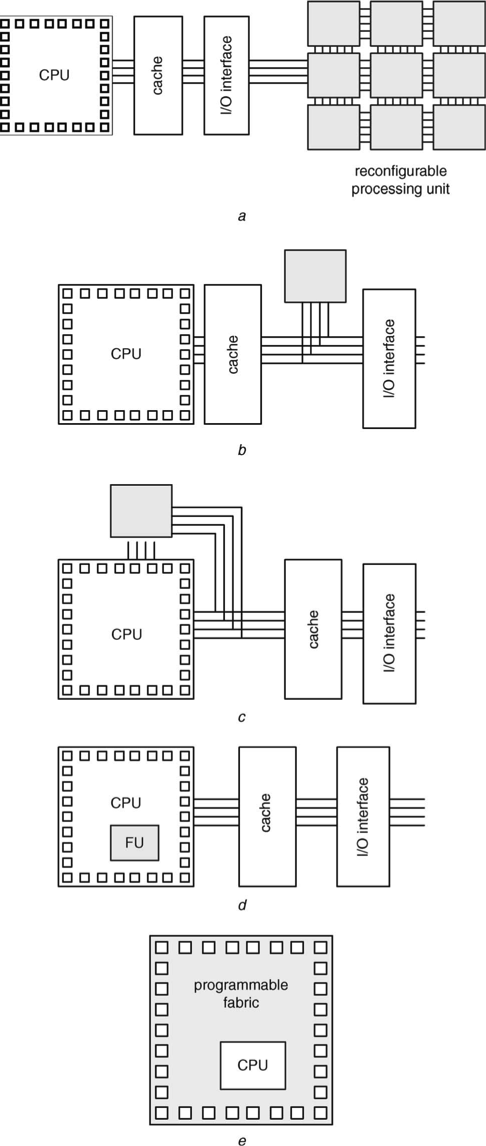
\includegraphics[width=0.5\textwidth]{./figs/fpga_cluster.png}
  \caption{Recofigurable systems; Adapted from \cite{compton2002reconfigurable}
  “(a) External stand-alone processing unit
(b) Attached processing unit
(c) Co-processor
(d) Reconfigurable functional unit
(e) Processor embedded in a reconfigurable fabric”
\cite{todman2005reconfigurable}}
  \label{fig:CE}
\end{figure}

In the design of a custom 64-FPGA cluster by Simon Moore et al. the existing PCI-Express connections present on Altera DE4 boards were converted to SATA3 connections achieving up to 6Gbps per connection between FPGAs with very low error rates (x10-15) \cite{moore2012bluehive}. This however, is a relatively high cost solution with custom board designs for the conversions and is required due to the un-structured requirement of interfacing for the neural-networking simulation. The error rate is also much higher than that required by our algorithm with simulations showing 94\% correct results even with 10\% error levels \cite{hu2012cmos}. 


The draw back of this communication structure however, was the all-to-all connection, allowing any FPGA to communicate with any other directly significantly increases the direct data throughput but has the cost of limiting the cluster to 64 chips. In this case the connections on the PCI-Express interface were at full utilisation making the cost of increasing cluster size prohibitive. One of the motivations of the DNA sequencing project is the ability to scale hardware to the required task. As a result the all-to-all approach shown here would be inappropriate. 


Another way of achieving this would be to have a common shared bus as seen in the top-level architecture of the Berkeley-Emulation-Engine (BEE2). This approach connected a 5-chip module to a 10 Gbps backbone network. This combines a hierarchical architecture with a high-speed network that also utilizes network-attached storage\cite{chang2005bee2}. The shared bus approach is an efficient solution on the assumption that board-to-board communication generally happens in random timing, if all boards were to attempt to communicate at the same time latency times would be unmanageable. In the case of this project a shared bus would be inefficient as the master FPGA receives data from the computer and then sends it out to each slave board. The result is practically all communication would ideally happen to several boards at the same time, causing latency issues. 

\section{Comparable DNA Sequencers}

As part of this project, identifying some relevant benchmarks for testing is necessary. These primarily fall into the category of CPU based algorithms as these are the simplest to implement and therefore the best to use for direct comparisons. A number of these systems exist and are available freely on the internet, a number of which have been used in sequencing tool-chains.

Velvet is a group of de novo DNA sequencing tools produced by Zerbino and Birney at the European Bioinformatics institute \cite{zerbino2008velvet}. Velvet was designed as a very short sequence assembler, using contiguous reads of around 35bp with very high coverage, this is significantly shorter than many other assemblers. This tool performs DNA assembly using a De Bruijn algorithm as well as several post-processing graph simplifications such as removing loops in the graph as well as forming blocks of reverse reads to account for reverse overlaps. This algorithm was implemented in C and during testing was run on a 64-bit linux machine. The authors conducted few tests on the algorithm, none of which discussed runtime. However the code has been made available on the European Bioinformatics webpage \cite{velvetdownload}.


The ABySS (Assembly BY Short Sequence) is a parallel tool for de novo sequencing \cite{simpson2009abyss}. The defining feature of the ABySS sequencer when it was built was that it was a truly parallel design where as sequencers such as velvet did not have the capacity. It is important to note however, with fast development in the field, systems such as Velvet have been adapted to support parallelism with tools such as OpenMPI. A common theme amongst these sequencing algorithms is that they incorporate the graph simplification and building, this is not true of the FPGA based comparison engine which makes analysis difficult. The main focus of the evaluation of ABySS in particular was the levels of correctness in the built graph, rather than the speed of the overlap comparison. This algorithm was also made available for public use on the British Columbia Genome Sciences Center (BCGSC) website \cite{ABYSSDOWNLOAD}.



A common method for sequencing short reads involves producing blocks of reads and reverse reads. This can be seen in both Velvet and tools like SSAKE, where blocks are formed of a read and its reverse. The reason for this is that the order start end of a read can not be guaranteed in the sequencing, and the algorithms commonly depend on the order of the sequence. As a result the blocking method is required so that reverse overlaps are not missed \cite{warren2007assembling}. This is commonly known as pair-end reads, as apposed to the normal single-end reads.The algorithm being implemented in this report relies exclusively on paired-end reads which are carried out automatically as part of the algorithm.



The SSAKE sequencer was implemented by Warren et al in 2006, and is also available on the BCGSC website \cite{SSAKEDOWNLOAD}. Benchmarks by the author of SSAKE achieved a 99.91\% correct sequence of the coronavirus from 476 016 reads of length 25 in a run time of 45.13 seconds on a dual core 2.2GHz AMD Opteron CPU. This will be a useful comparison to evaluate the work within this project \cite{warren2007assembling}.
\begin{figure}[h!]
\centering
  \includegraphics[width=0.65\textwidth,page=6]{./figs/comparisonlib.pdf}
  \caption{Comparison of Runtime and RAM usage for Sequencing Algorithms \cite{lin2011comparative}}
  \label{fig:comp}
\end{figure}
\pagebreak

A comparative study from the University of Shanghai for Science and Technology has produced some key comparisons between a set of sequencing algorithms. Running a variety of tests on algorithms including Velvet, ABySS, and SOAPdenovo run time and RAM usage was measured for a variety of genomes \cite{lin2011comparative}. This comparison is included in figure \ref{fig:comp}. The most important point to note from these comparisons is the long processing time required despite the hardware used. The hardware used in the test system was a cluster of 8 machines each with 2 quad-core processors. This is a highly-powerful setup and still required significant processing time for large sequence lengths. It does however, show a real application of DNA sequencer with highly relevant test data.


All the algorithms discussed in this section will be useful as comparable systems, it should be noted however that the hardware configurations used for these systems are often well beyond that used in this project. It may be necessary to factor this in when forming a comparison of these systems.







